\section{Appendix}
\label{sec:appendix}

\begin{figure}[htpb]
  \centering
  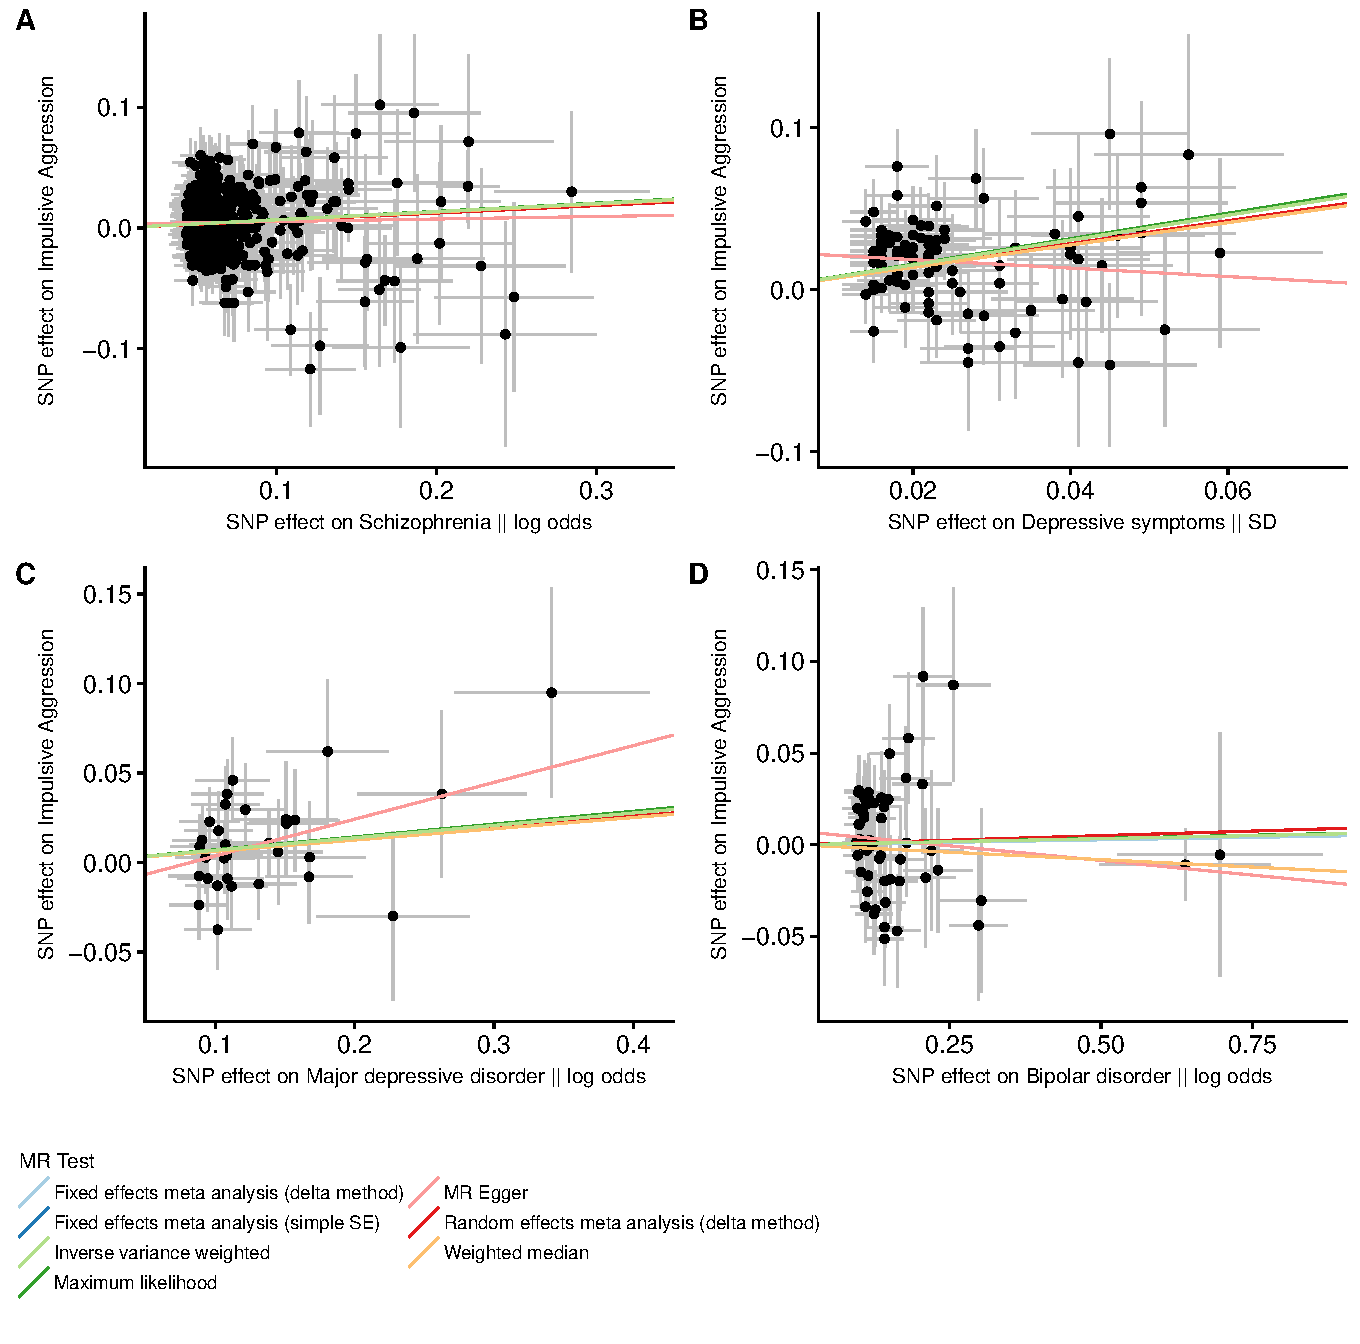
\includegraphics[width=0.7\linewidth]{ukb_psychiatric/figures/mr_aggression.pdf}
  \caption[Scatter Plot of the Causal Effects on Aggression]{
    Scatter plot of the Mendelian randomization between impulsive aggression and selected psychiatric disorders.
    Each panel displays the SNP effect of impulsive aggression against the log odds of a psychiatric disorder.
    Error bars display the standard error for impulsive aggression as well as psychiatric disorders.
    Furthermore, each line indicates the estimated causal effect of a specific psychiatric disorder on impulsive aggression for various methodologies.
    (A) Estimated causal effect of SZ on aggression.
    (B) Estimated causal effect of depressive symptoms on aggression.
    (C) Estimated causal effect of MDD on aggression.
    (D) Estimated causal effect of DP symptoms on aggression.
  }\label{fig:mr_aggression}
\end{figure}

\begin{figure}[htpb]
  \centering
  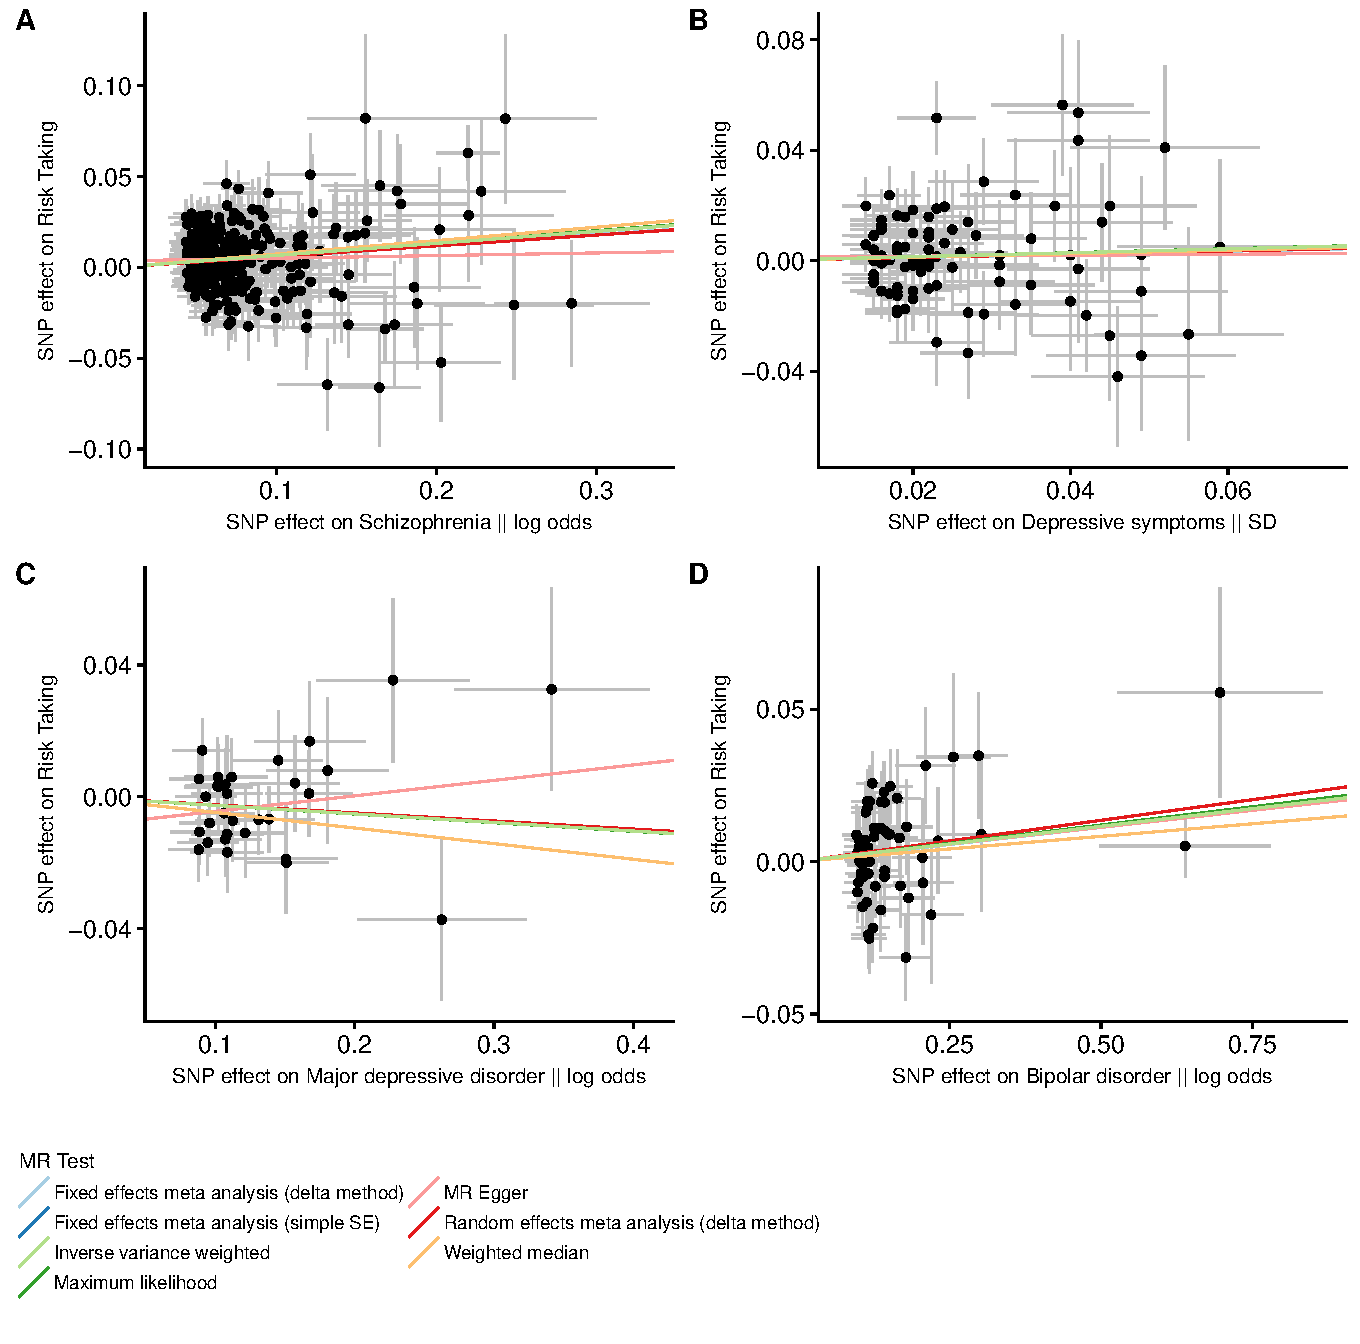
\includegraphics[width=0.7\linewidth]{ukb_psychiatric/figures/mr_risk.pdf}
  \caption[Scatter Plot of the Causal Effects on Risk Taking]{
    Scatter plot of the Mendelian randomization between risk taking and selected psychiatric disorders.
    Each panel displays the SNP effect of risk taking against the log odds of a psychiatric disorder.
    Error bars display the standard error for risk taking as well as psychiatric disorders.
    Furthermore, each line indicates the estimated causal effect of a specific psychiatric disorder on risk taking for various methodologies.
    (A) Estimated causal effect of SZ on risk taking.
    (B) Estimated causal effect of depressive symptoms on risk taking.
    (C) Estimated causal effect of MDD on risk taking.
    (D) Estimated causal effect of DP symptoms on risk taking.
  }\label{fig:mr_risk}
\end{figure}

\resizebox{1\linewidth}{!}{%latex.default(toprint, file = "aggression_instrument.tex", rowname = NULL,     center = "none", table.env = F)%
\toprule
\multicolumn{1}{c}{SNP}&\multicolumn{1}{c}{beta}&\multicolumn{1}{c}{se}&\multicolumn{1}{c}{N}&\multicolumn{1}{c}{pvalue}&\multicolumn{1}{c}{exposure}\\
\hline
rs10166548&$ 0.052$&$0.0115$&$ 82315$&$6.346e-06$&Schizophrenia\\
rs10273160&$ 0.069$&$0.0164$&$ 82315$&$2.513e-05$&Schizophrenia\\
rs1033394&$-0.058$&$0.0119$&$ 82315$&$9.757e-07$&Schizophrenia\\
rs10468795&$ 0.073$&$0.0173$&$ 82315$&$2.221e-05$&Schizophrenia\\
rs10520163&$ 0.061$&$0.0106$&$ 82315$&$1.020e-08$&Schizophrenia\\
rs10788251&$-0.081$&$0.0172$&$ 82315$&$2.372e-06$&Schizophrenia\\
rs10791097&$ 0.074$&$0.0106$&$ 82315$&$2.876e-12$&Schizophrenia\\
rs10832850&$ 0.050$&$0.0112$&$ 82315$&$1.079e-05$&Schizophrenia\\
rs10860152&$-0.049$&$0.0112$&$ 82315$&$9.575e-06$&Schizophrenia\\
rs10878577&$ 0.058$&$0.0124$&$ 82315$&$2.691e-06$&Schizophrenia\\
rs10891354&$-0.054$&$0.0116$&$ 82315$&$3.940e-06$&Schizophrenia\\
rs10926995&$-0.055$&$0.0109$&$ 82315$&$5.253e-07$&Schizophrenia\\
rs10954343&$ 0.065$&$0.0133$&$ 82315$&$1.219e-06$&Schizophrenia\\
rs10967586&$-0.085$&$0.0169$&$ 82315$&$4.749e-07$&Schizophrenia\\
rs11006253&$ 0.058$&$0.0121$&$ 82315$&$1.323e-06$&Schizophrenia\\
rs11027857&$ 0.063$&$0.0106$&$ 82315$&$3.210e-09$&Schizophrenia\\
rs1106568&$-0.069$&$0.0122$&$ 82315$&$1.145e-08$&Schizophrenia\\
rs11087338&$ 0.043$&$0.0106$&$ 82315$&$4.997e-05$&Schizophrenia\\
rs11122119&$ 0.047$&$0.0111$&$ 82315$&$2.446e-05$&Schizophrenia\\
rs1112586&$ 0.046$&$0.0110$&$ 82315$&$2.552e-05$&Schizophrenia\\
rs11144037&$ 0.067$&$0.0159$&$ 82315$&$2.177e-05$&Schizophrenia\\
rs111547017&$ 0.093$&$0.0190$&$ 82315$&$9.611e-07$&Schizophrenia\\
rs11209165&$-0.045$&$0.0109$&$ 82315$&$2.947e-05$&Schizophrenia\\
rs11210892&$-0.070$&$0.0112$&$ 82315$&$4.970e-10$&Schizophrenia\\
rs112221019&$-0.220$&$0.0528$&$ 82315$&$3.090e-05$&Schizophrenia\\
rs112902183&$ 0.188$&$0.0422$&$ 82315$&$8.426e-06$&Schizophrenia\\
rs113035110&$ 0.228$&$0.0529$&$ 82315$&$1.634e-05$&Schizophrenia\\
rs114042773&$-0.174$&$0.0360$&$ 82315$&$1.415e-06$&Schizophrenia\\
rs114834500&$ 0.113$&$0.0275$&$ 82315$&$3.725e-05$&Schizophrenia\\
rs115480152&$-0.141$&$0.0341$&$ 82315$&$3.781e-05$&Schizophrenia\\
rs11597992&$-0.053$&$0.0127$&$ 82315$&$2.625e-05$&Schizophrenia\\
rs11617058&$ 0.073$&$0.0147$&$ 82315$&$5.915e-07$&Schizophrenia\\
rs116250257&$-0.109$&$0.0266$&$ 82315$&$4.106e-05$&Schizophrenia\\
rs11625793&$-0.053$&$0.0109$&$ 82315$&$8.946e-07$&Schizophrenia\\
rs116606986&$ 0.243$&$0.0573$&$ 82315$&$2.230e-05$&Schizophrenia\\
rs116663126&$-0.082$&$0.0201$&$ 82315$&$4.474e-05$&Schizophrenia\\
rs11682175&$-0.074$&$0.0106$&$ 82315$&$2.543e-12$&Schizophrenia\\
rs11693094&$-0.073$&$0.0107$&$ 82315$&$7.131e-12$&Schizophrenia\\
rs116963868&$-0.175$&$0.0430$&$ 82315$&$4.454e-05$&Schizophrenia\\
rs117074560&$-0.157$&$0.0277$&$ 82315$&$1.661e-08$&Schizophrenia\\
rs11712112&$ 0.077$&$0.0173$&$ 82315$&$7.662e-06$&Schizophrenia\\
rs117435282&$-0.082$&$0.0199$&$ 82315$&$4.195e-05$&Schizophrenia\\
rs117578877&$ 0.136$&$0.0276$&$ 82315$&$8.814e-07$&Schizophrenia\\
rs117660826&$ 0.132$&$0.0313$&$ 82315$&$2.595e-05$&Schizophrenia\\
rs11785400&$ 0.053$&$0.0110$&$ 82315$&$1.524e-06$&Schizophrenia\\
rs117944154&$ 0.150$&$0.0343$&$ 82315$&$1.289e-05$&Schizophrenia\\
rs11807834&$ 0.060$&$0.0125$&$ 82315$&$1.763e-06$&Schizophrenia\\
rs11813412&$-0.073$&$0.0176$&$ 82315$&$2.977e-05$&Schizophrenia\\
rs12129573&$ 0.069$&$0.0110$&$ 82315$&$2.346e-10$&Schizophrenia\\
rs12129719&$ 0.056$&$0.0109$&$ 82315$&$2.896e-07$&Schizophrenia\\
rs12237911&$ 0.113$&$0.0251$&$ 82315$&$6.440e-06$&Schizophrenia\\
rs12326186&$-0.055$&$0.0121$&$ 82315$&$6.490e-06$&Schizophrenia\\
rs12431410&$-0.056$&$0.0110$&$ 82315$&$4.217e-07$&Schizophrenia\\
rs12478153&$-0.102$&$0.0252$&$ 82315$&$4.862e-05$&Schizophrenia\\
rs12510251&$ 0.071$&$0.0134$&$ 82315$&$1.430e-07$&Schizophrenia\\
rs12541792&$-0.049$&$0.0119$&$ 82315$&$3.250e-05$&Schizophrenia\\
rs1265876&$ 0.054$&$0.0124$&$ 82315$&$1.243e-05$&Schizophrenia\\
rs12691307&$ 0.071$&$0.0110$&$ 82315$&$1.298e-10$&Schizophrenia\\
rs12704290&$-0.107$&$0.0165$&$ 82315$&$1.037e-10$&Schizophrenia\\
rs12723316&$-0.071$&$0.0152$&$ 82315$&$3.309e-06$&Schizophrenia\\
rs12826178&$-0.168$&$0.0243$&$ 82315$&$5.297e-12$&Schizophrenia\\
rs12883788&$ 0.057$&$0.0112$&$ 82315$&$3.421e-07$&Schizophrenia\\
rs12887734&$ 0.087$&$0.0117$&$ 82315$&$1.172e-13$&Schizophrenia\\
rs12903146&$ 0.065$&$0.0106$&$ 82315$&$1.038e-09$&Schizophrenia\\
rs12914626&$-0.058$&$0.0116$&$ 82315$&$5.186e-07$&Schizophrenia\\
rs12938078&$ 0.062$&$0.0138$&$ 82315$&$6.992e-06$&Schizophrenia\\
rs12955051&$-0.045$&$0.0112$&$ 82315$&$4.939e-05$&Schizophrenia\\
rs12991836&$-0.053$&$0.0110$&$ 82315$&$1.747e-06$&Schizophrenia\\
rs12997796&$ 0.064$&$0.0137$&$ 82315$&$3.077e-06$&Schizophrenia\\
rs13006127&$-0.043$&$0.0106$&$ 82315$&$4.345e-05$&Schizophrenia\\
rs13013484&$ 0.050$&$0.0117$&$ 82315$&$1.920e-05$&Schizophrenia\\
rs13074132&$ 0.056$&$0.0113$&$ 82315$&$6.940e-07$&Schizophrenia\\
rs13078331&$ 0.051$&$0.0118$&$ 82315$&$1.579e-05$&Schizophrenia\\
rs13217619&$ 0.220$&$0.0195$&$ 82315$&$1.435e-29$&Schizophrenia\\
rs13240464&$ 0.081$&$0.0112$&$ 82315$&$6.162e-13$&Schizophrenia\\
rs13276960&$-0.064$&$0.0141$&$ 82315$&$5.325e-06$&Schizophrenia\\
rs1329313&$ 0.054$&$0.0107$&$ 82315$&$3.410e-07$&Schizophrenia\\
rs13293831&$ 0.067$&$0.0148$&$ 82315$&$5.062e-06$&Schizophrenia\\
rs1339227&$-0.060$&$0.0111$&$ 82315$&$6.860e-08$&Schizophrenia\\
rs1360695&$ 0.055$&$0.0109$&$ 82315$&$4.891e-07$&Schizophrenia\\
rs140130327&$ 0.248$&$0.0495$&$ 82315$&$5.326e-07$&Schizophrenia\\
rs140505938&$-0.091$&$0.0148$&$ 82315$&$9.337e-10$&Schizophrenia\\
rs1422755&$-0.046$&$0.0108$&$ 82315$&$2.288e-05$&Schizophrenia\\
rs145607970&$-0.164$&$0.0256$&$ 82315$&$1.345e-10$&Schizophrenia\\
rs147897924&$-0.063$&$0.0136$&$ 82315$&$3.479e-06$&Schizophrenia\\
rs1482292&$-0.082$&$0.0172$&$ 82315$&$1.863e-06$&Schizophrenia\\
rs149110600&$ 0.109$&$0.0227$&$ 82315$&$1.691e-06$&Schizophrenia\\
rs149818&$ 0.044$&$0.0106$&$ 82315$&$2.838e-05$&Schizophrenia\\
rs1498232&$ 0.070$&$0.0115$&$ 82315$&$1.284e-09$&Schizophrenia\\
rs1501357&$-0.077$&$0.0134$&$ 82315$&$1.236e-08$&Schizophrenia\\
rs1509378&$ 0.062$&$0.0115$&$ 82315$&$8.371e-08$&Schizophrenia\\
rs151260629&$-0.136$&$0.0332$&$ 82315$&$4.255e-05$&Schizophrenia\\
rs1518933&$ 0.052$&$0.0106$&$ 82315$&$7.509e-07$&Schizophrenia\\
rs1524480&$-0.062$&$0.0134$&$ 82315$&$4.046e-06$&Schizophrenia\\
rs1583830&$-0.047$&$0.0109$&$ 82315$&$1.539e-05$&Schizophrenia\\
rs16830627&$ 0.083$&$0.0171$&$ 82315$&$1.311e-06$&Schizophrenia\\
rs16867576&$ 0.096$&$0.0169$&$ 82315$&$1.358e-08$&Schizophrenia\\
rs16937&$ 0.056$&$0.0113$&$ 82315$&$8.691e-07$&Schizophrenia\\
rs16942745&$ 0.123$&$0.0294$&$ 82315$&$3.102e-05$&Schizophrenia\\
rs1702294&$-0.116$&$0.0137$&$ 82315$&$2.794e-17$&Schizophrenia\\
rs17039547&$ 0.051$&$0.0117$&$ 82315$&$1.586e-05$&Schizophrenia\\
rs1717776&$-0.052$&$0.0110$&$ 82315$&$2.534e-06$&Schizophrenia\\
rs17194490&$ 0.097$&$0.0148$&$ 82315$&$4.865e-11$&Schizophrenia\\
rs17432316&$ 0.060$&$0.0127$&$ 82315$&$2.267e-06$&Schizophrenia\\
rs17731&$ 0.052$&$0.0109$&$ 82315$&$2.154e-06$&Schizophrenia\\
rs17765037&$ 0.049$&$0.0121$&$ 82315$&$4.643e-05$&Schizophrenia\\
rs183823891&$ 0.071$&$0.0135$&$ 82315$&$1.339e-07$&Schizophrenia\\
rs1863824&$-0.050$&$0.0109$&$ 82315$&$5.548e-06$&Schizophrenia\\
rs187046000&$ 0.178$&$0.0428$&$ 82315$&$3.334e-05$&Schizophrenia\\
rs1914395&$ 0.102$&$0.0204$&$ 82315$&$5.199e-07$&Schizophrenia\\
rs1927813&$-0.046$&$0.0113$&$ 82315$&$3.876e-05$&Schizophrenia\\
rs1939214&$ 0.077$&$0.0144$&$ 82315$&$8.882e-08$&Schizophrenia\\
rs1951329&$ 0.044$&$0.0107$&$ 82315$&$3.067e-05$&Schizophrenia\\
rs1979406&$-0.078$&$0.0188$&$ 82315$&$3.171e-05$&Schizophrenia\\
rs1999512&$-0.052$&$0.0124$&$ 82315$&$2.554e-05$&Schizophrenia\\
rs2007044&$-0.092$&$0.0108$&$ 82315$&$2.625e-17$&Schizophrenia\\
rs2008905&$ 0.049$&$0.0109$&$ 82315$&$8.009e-06$&Schizophrenia\\
rs2026714&$-0.056$&$0.0107$&$ 82315$&$1.877e-07$&Schizophrenia\\
rs2053079&$-0.073$&$0.0124$&$ 82315$&$3.789e-09$&Schizophrenia\\
rs2055388&$-0.127$&$0.0302$&$ 82315$&$2.530e-05$&Schizophrenia\\
rs2068012&$-0.069$&$0.0126$&$ 82315$&$4.142e-08$&Schizophrenia\\
rs2068485&$ 0.044$&$0.0106$&$ 82315$&$3.436e-05$&Schizophrenia\\
rs207282&$ 0.053$&$0.0113$&$ 82315$&$2.762e-06$&Schizophrenia\\
rs2077316&$ 0.119$&$0.0263$&$ 82315$&$6.385e-06$&Schizophrenia\\
rs2077586&$ 0.065$&$0.0124$&$ 82315$&$1.534e-07$&Schizophrenia\\
rs2094900&$ 0.052$&$0.0107$&$ 82315$&$1.269e-06$&Schizophrenia\\
rs2108349&$ 0.047$&$0.0114$&$ 82315$&$4.188e-05$&Schizophrenia\\
rs2137272&$-0.047$&$0.0107$&$ 82315$&$1.141e-05$&Schizophrenia\\
rs216452&$ 0.050$&$0.0113$&$ 82315$&$1.120e-05$&Schizophrenia\\
rs2181872&$-0.053$&$0.0124$&$ 82315$&$1.967e-05$&Schizophrenia\\
rs2185077&$ 0.072$&$0.0155$&$ 82315$&$3.324e-06$&Schizophrenia\\
rs2189246&$ 0.048$&$0.0107$&$ 82315$&$7.164e-06$&Schizophrenia\\
rs2205298&$-0.056$&$0.0124$&$ 82315$&$5.255e-06$&Schizophrenia\\
rs223369&$ 0.053$&$0.0125$&$ 82315$&$2.501e-05$&Schizophrenia\\
rs2247419&$-0.054$&$0.0107$&$ 82315$&$4.305e-07$&Schizophrenia\\
rs227932&$-0.085$&$0.0167$&$ 82315$&$3.757e-07$&Schizophrenia\\
rs2285217&$-0.049$&$0.0109$&$ 82315$&$7.015e-06$&Schizophrenia\\
rs2304389&$ 0.073$&$0.0145$&$ 82315$&$5.478e-07$&Schizophrenia\\
rs2381411&$-0.046$&$0.0110$&$ 82315$&$2.913e-05$&Schizophrenia\\
rs238783&$-0.051$&$0.0114$&$ 82315$&$7.692e-06$&Schizophrenia\\
rs2413045&$ 0.062$&$0.0144$&$ 82315$&$1.455e-05$&Schizophrenia\\
rs2428161&$-0.047$&$0.0106$&$ 82315$&$1.100e-05$&Schizophrenia\\
rs248083&$ 0.051$&$0.0113$&$ 82315$&$6.056e-06$&Schizophrenia\\
rs2491015&$-0.049$&$0.0112$&$ 82315$&$1.239e-05$&Schizophrenia\\
rs2496034&$-0.065$&$0.0143$&$ 82315$&$5.200e-06$&Schizophrenia\\
rs2507860&$ 0.052$&$0.0113$&$ 82315$&$3.245e-06$&Schizophrenia\\
rs2514218&$-0.072$&$0.0116$&$ 82315$&$4.091e-10$&Schizophrenia\\
rs2526882&$-0.057$&$0.0111$&$ 82315$&$3.165e-07$&Schizophrenia\\
rs2532197&$-0.050$&$0.0113$&$ 82315$&$1.189e-05$&Schizophrenia\\
rs2535627&$ 0.070$&$0.0106$&$ 82315$&$3.956e-11$&Schizophrenia\\
rs2540277&$-0.099$&$0.0221$&$ 82315$&$7.789e-06$&Schizophrenia\\
rs2563297&$-0.052$&$0.0106$&$ 82315$&$8.553e-07$&Schizophrenia\\
rs2693698&$-0.063$&$0.0111$&$ 82315$&$1.375e-08$&Schizophrenia\\
rs27419&$-0.049$&$0.0111$&$ 82315$&$9.917e-06$&Schizophrenia\\
rs2796441&$-0.056$&$0.0109$&$ 82315$&$2.214e-07$&Schizophrenia\\
rs2828478&$ 0.057$&$0.0113$&$ 82315$&$5.261e-07$&Schizophrenia\\
rs28375034&$-0.075$&$0.0155$&$ 82315$&$1.234e-06$&Schizophrenia\\
rs2843744&$ 0.050$&$0.0113$&$ 82315$&$8.067e-06$&Schizophrenia\\
rs28633584&$-0.057$&$0.0141$&$ 82315$&$4.976e-05$&Schizophrenia\\
rs28735056&$-0.054$&$0.0110$&$ 82315$&$1.068e-06$&Schizophrenia\\
rs2876825&$ 0.057$&$0.0135$&$ 82315$&$2.147e-05$&Schizophrenia\\
rs2905426&$-0.065$&$0.0112$&$ 82315$&$6.921e-09$&Schizophrenia\\
rs2909457&$-0.059$&$0.0108$&$ 82315$&$4.375e-08$&Schizophrenia\\
rs2945232&$-0.061$&$0.0108$&$ 82315$&$2.034e-08$&Schizophrenia\\
rs2956973&$-0.046$&$0.0108$&$ 82315$&$2.114e-05$&Schizophrenia\\
rs2973155&$-0.067$&$0.0110$&$ 82315$&$1.016e-09$&Schizophrenia\\
rs301797&$ 0.068$&$0.0115$&$ 82315$&$2.724e-09$&Schizophrenia\\
rs302010&$-0.069$&$0.0142$&$ 82315$&$1.312e-06$&Schizophrenia\\
rs306206&$ 0.064$&$0.0122$&$ 82315$&$1.978e-07$&Schizophrenia\\
rs306375&$ 0.048$&$0.0114$&$ 82315$&$2.938e-05$&Schizophrenia\\
rs328764&$ 0.060$&$0.0140$&$ 82315$&$1.636e-05$&Schizophrenia\\
rs34102591&$-0.069$&$0.0136$&$ 82315$&$4.066e-07$&Schizophrenia\\
rs34411452&$ 0.062$&$0.0137$&$ 82315$&$6.083e-06$&Schizophrenia\\
rs34753377&$ 0.064$&$0.0121$&$ 82315$&$1.061e-07$&Schizophrenia\\
rs34796896&$-0.086$&$0.0132$&$ 82315$&$6.234e-11$&Schizophrenia\\
rs35123781&$-0.054$&$0.0114$&$ 82315$&$1.717e-06$&Schizophrenia\\
rs35225200&$-0.145$&$0.0203$&$ 82315$&$9.562e-13$&Schizophrenia\\
rs352766&$-0.070$&$0.0162$&$ 82315$&$1.537e-05$&Schizophrenia\\
rs36068923&$-0.084$&$0.0130$&$ 82315$&$1.045e-10$&Schizophrenia\\
rs36109662&$-0.079$&$0.0178$&$ 82315$&$8.659e-06$&Schizophrenia\\
rs3735025&$ 0.064$&$0.0110$&$ 82315$&$7.752e-09$&Schizophrenia\\
rs3741434&$-0.070$&$0.0169$&$ 82315$&$3.529e-05$&Schizophrenia\\
rs3757859&$-0.063$&$0.0145$&$ 82315$&$1.208e-05$&Schizophrenia\\
rs3770752&$ 0.054$&$0.0114$&$ 82315$&$2.631e-06$&Schizophrenia\\
rs3798869&$-0.065$&$0.0106$&$ 82315$&$1.153e-09$&Schizophrenia\\
rs3806573&$ 0.068$&$0.0160$&$ 82315$&$2.262e-05$&Schizophrenia\\
rs3849046&$ 0.063$&$0.0107$&$ 82315$&$4.833e-09$&Schizophrenia\\
rs4084594&$ 0.052$&$0.0111$&$ 82315$&$2.277e-06$&Schizophrenia\\
rs4129585&$ 0.078$&$0.0107$&$ 82315$&$2.028e-13$&Schizophrenia\\
rs41314284&$ 0.089$&$0.0190$&$ 82315$&$3.068e-06$&Schizophrenia\\
rs427230&$ 0.116$&$0.0211$&$ 82315$&$4.028e-08$&Schizophrenia\\
rs4273100&$ 0.090$&$0.0182$&$ 82315$&$7.772e-07$&Schizophrenia\\
rs4330281&$-0.059$&$0.0108$&$ 82315$&$5.505e-08$&Schizophrenia\\
rs4388249&$ 0.072$&$0.0135$&$ 82315$&$1.025e-07$&Schizophrenia\\
rs4391122&$-0.079$&$0.0107$&$ 82315$&$1.734e-13$&Schizophrenia\\
rs4402447&$ 0.087$&$0.0215$&$ 82315$&$4.861e-05$&Schizophrenia\\
rs4523957&$ 0.068$&$0.0112$&$ 82315$&$1.040e-09$&Schizophrenia\\
rs4533758&$-0.047$&$0.0112$&$ 82315$&$2.460e-05$&Schizophrenia\\
rs4626214&$-0.054$&$0.0109$&$ 82315$&$6.068e-07$&Schizophrenia\\
rs4648845&$ 0.069$&$0.0117$&$ 82315$&$4.033e-09$&Schizophrenia\\
rs4685497&$-0.058$&$0.0140$&$ 82315$&$3.287e-05$&Schizophrenia\\
rs4702&$-0.078$&$0.0112$&$ 82315$&$2.298e-12$&Schizophrenia\\
rs4741507&$ 0.057$&$0.0133$&$ 82315$&$2.009e-05$&Schizophrenia\\
rs4746299&$ 0.060$&$0.0146$&$ 82315$&$4.336e-05$&Schizophrenia\\
rs4766428&$ 0.068$&$0.0111$&$ 82315$&$7.093e-10$&Schizophrenia\\
rs4814463&$-0.052$&$0.0126$&$ 82315$&$3.204e-05$&Schizophrenia\\
rs4820504&$ 0.052$&$0.0120$&$ 82315$&$1.356e-05$&Schizophrenia\\
rs4823690&$ 0.046$&$0.0112$&$ 82315$&$3.645e-05$&Schizophrenia\\
rs4876021&$-0.073$&$0.0177$&$ 82315$&$3.202e-05$&Schizophrenia\\
rs4963432&$ 0.053$&$0.0109$&$ 82315$&$1.312e-06$&Schizophrenia\\
rs524489&$-0.048$&$0.0109$&$ 82315$&$9.350e-06$&Schizophrenia\\
rs524732&$ 0.060$&$0.0128$&$ 82315$&$3.172e-06$&Schizophrenia\\
rs55675132&$-0.056$&$0.0121$&$ 82315$&$3.274e-06$&Schizophrenia\\
rs55711779&$ 0.049$&$0.0120$&$ 82315$&$4.384e-05$&Schizophrenia\\
rs55771921&$ 0.061$&$0.0140$&$ 82315$&$1.355e-05$&Schizophrenia\\
rs55895733&$ 0.068$&$0.0154$&$ 82315$&$1.153e-05$&Schizophrenia\\
rs56145559&$ 0.071$&$0.0132$&$ 82315$&$8.424e-08$&Schizophrenia\\
rs56775891&$ 0.061$&$0.0118$&$ 82315$&$2.173e-07$&Schizophrenia\\
rs56873913&$ 0.067$&$0.0129$&$ 82315$&$2.188e-07$&Schizophrenia\\
rs58120505&$ 0.081$&$0.0108$&$ 82315$&$6.426e-14$&Schizophrenia\\
rs59979824&$-0.066$&$0.0116$&$ 82315$&$1.079e-08$&Schizophrenia\\
rs60558575&$-0.094$&$0.0231$&$ 82315$&$4.608e-05$&Schizophrenia\\
rs6065094&$-0.074$&$0.0113$&$ 82315$&$5.519e-11$&Schizophrenia\\
rs60710459&$ 0.081$&$0.0169$&$ 82315$&$1.959e-06$&Schizophrenia\\
rs6096217&$-0.046$&$0.0110$&$ 82315$&$3.245e-05$&Schizophrenia\\
rs6137162&$ 0.061$&$0.0115$&$ 82315$&$1.215e-07$&Schizophrenia\\
rs61847307&$-0.063$&$0.0121$&$ 82315$&$2.082e-07$&Schizophrenia\\
rs61878685&$-0.121$&$0.0280$&$ 82315$&$1.526e-05$&Schizophrenia\\
rs61921611&$-0.052$&$0.0116$&$ 82315$&$7.086e-06$&Schizophrenia\\
rs62002390&$ 0.119$&$0.0280$&$ 82315$&$2.187e-05$&Schizophrenia\\
rs62039478&$ 0.074$&$0.0174$&$ 82315$&$1.919e-05$&Schizophrenia\\
rs62064224&$-0.050$&$0.0110$&$ 82315$&$5.717e-06$&Schizophrenia\\
rs62125166&$ 0.069$&$0.0137$&$ 82315$&$4.382e-07$&Schizophrenia\\
rs62442053&$-0.083$&$0.0193$&$ 82315$&$1.792e-05$&Schizophrenia\\
rs629280&$ 0.058$&$0.0138$&$ 82315$&$3.051e-05$&Schizophrenia\\
rs634940&$ 0.059$&$0.0124$&$ 82315$&$2.267e-06$&Schizophrenia\\
rs6430095&$ 0.081$&$0.0142$&$ 82315$&$1.209e-08$&Schizophrenia\\
rs6430491&$-0.064$&$0.0134$&$ 82315$&$1.612e-06$&Schizophrenia\\
rs643949&$-0.114$&$0.0247$&$ 82315$&$3.753e-06$&Schizophrenia\\
rs6468049&$ 0.049$&$0.0109$&$ 82315$&$6.632e-06$&Schizophrenia\\
rs648516&$ 0.055$&$0.0111$&$ 82315$&$7.217e-07$&Schizophrenia\\
rs6500602&$ 0.060$&$0.0116$&$ 82315$&$2.792e-07$&Schizophrenia\\
rs6510698&$-0.065$&$0.0135$&$ 82315$&$1.263e-06$&Schizophrenia\\
rs6518257&$-0.055$&$0.0117$&$ 82315$&$2.508e-06$&Schizophrenia\\
rs6549963&$ 0.052$&$0.0109$&$ 82315$&$1.702e-06$&Schizophrenia\\
rs6670165&$ 0.071$&$0.0135$&$ 82315$&$1.156e-07$&Schizophrenia\\
rs67032849&$-0.048$&$0.0113$&$ 82315$&$1.994e-05$&Schizophrenia\\
rs6704768&$-0.074$&$0.0106$&$ 82315$&$3.148e-12$&Schizophrenia\\
rs674001&$-0.067$&$0.0164$&$ 82315$&$3.886e-05$&Schizophrenia\\
rs6758546&$ 0.072$&$0.0166$&$ 82315$&$1.418e-05$&Schizophrenia\\
rs6788179&$-0.079$&$0.0170$&$ 82315$&$3.778e-06$&Schizophrenia\\
rs679087&$-0.061$&$0.0113$&$ 82315$&$7.058e-08$&Schizophrenia\\
rs6810442&$-0.076$&$0.0177$&$ 82315$&$1.584e-05$&Schizophrenia\\
rs68162274&$ 0.073$&$0.0171$&$ 82315$&$1.919e-05$&Schizophrenia\\
rs6825268&$-0.055$&$0.0111$&$ 82315$&$7.443e-07$&Schizophrenia\\
rs6846507&$-0.078$&$0.0192$&$ 82315$&$4.571e-05$&Schizophrenia\\
rs684699&$ 0.053$&$0.0122$&$ 82315$&$1.332e-05$&Schizophrenia\\
rs6919939&$ 0.054$&$0.0116$&$ 82315$&$4.198e-06$&Schizophrenia\\
rs6984242&$-0.064$&$0.0107$&$ 82315$&$1.758e-09$&Schizophrenia\\
rs698671&$-0.052$&$0.0116$&$ 82315$&$9.233e-06$&Schizophrenia\\
rs7008026&$-0.067$&$0.0147$&$ 82315$&$4.728e-06$&Schizophrenia\\
rs7095279&$ 0.046$&$0.0106$&$ 82315$&$1.608e-05$&Schizophrenia\\
rs71316430&$ 0.121$&$0.0278$&$ 82315$&$1.276e-05$&Schizophrenia\\
rs7193419&$ 0.060$&$0.0106$&$ 82315$&$1.588e-08$&Schizophrenia\\
rs7194676&$-0.059$&$0.0137$&$ 82315$&$1.406e-05$&Schizophrenia\\
rs7257451&$-0.048$&$0.0116$&$ 82315$&$4.059e-05$&Schizophrenia\\
rs7267348&$-0.064$&$0.0121$&$ 82315$&$1.182e-07$&Schizophrenia\\
rs72983260&$-0.058$&$0.0139$&$ 82315$&$2.858e-05$&Schizophrenia\\
rs72986630&$ 0.145$&$0.0266$&$ 82315$&$4.636e-08$&Schizophrenia\\
rs73060317&$ 0.061$&$0.0124$&$ 82315$&$6.604e-07$&Schizophrenia\\
rs73185299&$ 0.055$&$0.0116$&$ 82315$&$1.836e-06$&Schizophrenia\\
rs7322886&$ 0.045$&$0.0109$&$ 82315$&$3.597e-05$&Schizophrenia\\
rs73229090&$-0.099$&$0.0177$&$ 82315$&$1.952e-08$&Schizophrenia\\
rs7372960&$ 0.067$&$0.0127$&$ 82315$&$1.249e-07$&Schizophrenia\\
rs7405404&$ 0.078$&$0.0125$&$ 82315$&$3.925e-10$&Schizophrenia\\
rs7432375&$-0.071$&$0.0109$&$ 82315$&$5.274e-11$&Schizophrenia\\
rs75156607&$-0.155$&$0.0360$&$ 82315$&$1.588e-05$&Schizophrenia\\
rs7521492&$ 0.055$&$0.0110$&$ 82315$&$5.641e-07$&Schizophrenia\\
rs7521837&$ 0.059$&$0.0128$&$ 82315$&$5.128e-06$&Schizophrenia\\
rs7523273&$ 0.060$&$0.0115$&$ 82315$&$1.609e-07$&Schizophrenia\\
rs75267292&$-0.155$&$0.0303$&$ 82315$&$3.112e-07$&Schizophrenia\\
rs7551345&$ 0.064$&$0.0138$&$ 82315$&$3.509e-06$&Schizophrenia\\
rs7577463&$-0.061$&$0.0123$&$ 82315$&$5.487e-07$&Schizophrenia\\
rs7577690&$ 0.055$&$0.0115$&$ 82315$&$1.598e-06$&Schizophrenia\\
rs758129&$-0.051$&$0.0111$&$ 82315$&$3.956e-06$&Schizophrenia\\
rs75947768&$ 0.111$&$0.0262$&$ 82315$&$2.428e-05$&Schizophrenia\\
rs75968099&$ 0.079$&$0.0113$&$ 82315$&$3.386e-12$&Schizophrenia\\
rs7599488&$-0.055$&$0.0108$&$ 82315$&$3.114e-07$&Schizophrenia\\
rs7601312&$-0.057$&$0.0105$&$ 82315$&$6.434e-08$&Schizophrenia\\
rs761840&$ 0.049$&$0.0115$&$ 82315$&$1.985e-05$&Schizophrenia\\
rs76405237&$-0.137$&$0.0290$&$ 82315$&$2.301e-06$&Schizophrenia\\
rs76456399&$ 0.186$&$0.0413$&$ 82315$&$6.562e-06$&Schizophrenia\\
rs76503615&$ 0.104$&$0.0235$&$ 82315$&$9.248e-06$&Schizophrenia\\
rs77071458&$-0.064$&$0.0146$&$ 82315$&$1.110e-05$&Schizophrenia\\
rs7710182&$-0.056$&$0.0131$&$ 82315$&$1.856e-05$&Schizophrenia\\
rs77149735&$ 0.285$&$0.0485$&$ 82315$&$4.404e-09$&Schizophrenia\\
rs77206190&$ 0.165$&$0.0365$&$ 82315$&$6.560e-06$&Schizophrenia\\
rs7742212&$ 0.047$&$0.0107$&$ 82315$&$1.113e-05$&Schizophrenia\\
rs775018&$-0.050$&$0.0110$&$ 82315$&$5.674e-06$&Schizophrenia\\
rs7779018&$ 0.063$&$0.0118$&$ 82315$&$9.695e-08$&Schizophrenia\\
rs77943030&$-0.070$&$0.0160$&$ 82315$&$1.419e-05$&Schizophrenia\\
rs7811528&$-0.068$&$0.0149$&$ 82315$&$4.772e-06$&Schizophrenia\\
rs7819570&$ 0.077$&$0.0137$&$ 82315$&$1.899e-08$&Schizophrenia\\
rs78294120&$-0.202$&$0.0472$&$ 82315$&$1.917e-05$&Schizophrenia\\
rs78381888&$ 0.083$&$0.0158$&$ 82315$&$1.501e-07$&Schizophrenia\\
rs78392994&$ 0.089$&$0.0195$&$ 82315$&$5.048e-06$&Schizophrenia\\
rs7846730&$-0.044$&$0.0105$&$ 82315$&$2.595e-05$&Schizophrenia\\
rs78774248&$ 0.074$&$0.0167$&$ 82315$&$8.087e-06$&Schizophrenia\\
rs7893279&$ 0.113$&$0.0171$&$ 82315$&$3.562e-11$&Schizophrenia\\
rs7899469&$ 0.050$&$0.0116$&$ 82315$&$1.397e-05$&Schizophrenia\\
rs79090407&$ 0.118$&$0.0244$&$ 82315$&$1.451e-06$&Schizophrenia\\
rs79193624&$ 0.203$&$0.0374$&$ 82315$&$5.978e-08$&Schizophrenia\\
rs7934083&$-0.056$&$0.0109$&$ 82315$&$2.415e-07$&Schizophrenia\\
rs79445414&$-0.145$&$0.0274$&$ 82315$&$1.364e-07$&Schizophrenia\\
rs7951870&$-0.092$&$0.0142$&$ 82315$&$8.253e-11$&Schizophrenia\\
rs7978185&$-0.044$&$0.0108$&$ 82315$&$4.684e-05$&Schizophrenia\\
rs79943431&$ 0.115$&$0.0256$&$ 82315$&$6.821e-06$&Schizophrenia\\
rs8016982&$-0.049$&$0.0111$&$ 82315$&$9.607e-06$&Schizophrenia\\
rs8025470&$ 0.095$&$0.0216$&$ 82315$&$1.168e-05$&Schizophrenia\\
rs8042374&$ 0.087$&$0.0124$&$ 82315$&$1.865e-12$&Schizophrenia\\
rs8044995&$ 0.078$&$0.0141$&$ 82315$&$3.268e-08$&Schizophrenia\\
rs8066384&$-0.058$&$0.0119$&$ 82315$&$1.124e-06$&Schizophrenia\\
rs8072321&$ 0.051$&$0.0109$&$ 82315$&$3.560e-06$&Schizophrenia\\
rs8099121&$ 0.060$&$0.0131$&$ 82315$&$4.810e-06$&Schizophrenia\\
rs811043&$ 0.054$&$0.0117$&$ 82315$&$3.584e-06$&Schizophrenia\\
rs8112050&$-0.048$&$0.0116$&$ 82315$&$4.448e-05$&Schizophrenia\\
rs8127118&$-0.049$&$0.0110$&$ 82315$&$6.339e-06$&Schizophrenia\\
rs8139773&$-0.071$&$0.0111$&$ 82315$&$1.356e-10$&Schizophrenia\\
rs8181679&$ 0.050$&$0.0109$&$ 82315$&$4.238e-06$&Schizophrenia\\
rs832187&$-0.061$&$0.0109$&$ 82315$&$2.584e-08$&Schizophrenia\\
rs9310732&$ 0.052$&$0.0110$&$ 82315$&$1.981e-06$&Schizophrenia\\
rs9316337&$-0.051$&$0.0107$&$ 82315$&$1.713e-06$&Schizophrenia\\
rs9330316&$ 0.062$&$0.0115$&$ 82315$&$7.687e-08$&Schizophrenia\\
rs9341835&$-0.052$&$0.0109$&$ 82315$&$1.687e-06$&Schizophrenia\\
rs9362395&$ 0.114$&$0.0226$&$ 82315$&$4.203e-07$&Schizophrenia\\
rs9398171&$-0.064$&$0.0115$&$ 82315$&$3.373e-08$&Schizophrenia\\
rs9420&$ 0.061$&$0.0113$&$ 82315$&$6.652e-08$&Schizophrenia\\
rs949025&$ 0.059$&$0.0125$&$ 82315$&$2.027e-06$&Schizophrenia\\
rs9584154&$ 0.055$&$0.0111$&$ 82315$&$7.067e-07$&Schizophrenia\\
rs9636107&$-0.076$&$0.0107$&$ 82315$&$9.091e-13$&Schizophrenia\\
rs9669686&$ 0.047$&$0.0107$&$ 82315$&$1.276e-05$&Schizophrenia\\
rs9695226&$-0.059$&$0.0115$&$ 82315$&$2.518e-07$&Schizophrenia\\
rs975752&$ 0.087$&$0.0184$&$ 82315$&$2.524e-06$&Schizophrenia\\
rs987335&$ 0.044$&$0.0107$&$ 82315$&$3.768e-05$&Schizophrenia\\
rs9873519&$ 0.046$&$0.0106$&$ 82315$&$1.385e-05$&Schizophrenia\\
rs9876310&$-0.072$&$0.0167$&$ 82315$&$1.614e-05$&Schizophrenia\\
rs9903469&$-0.070$&$0.0167$&$ 82315$&$2.757e-05$&Schizophrenia\\
rs10011311&$ 0.027$&$0.0060$&$161460$&$8.137e-06$&Depressive symptoms\\
rs10030686&$ 0.018$&$0.0040$&$161460$&$1.074e-05$&Depressive symptoms\\
rs10106565&$ 0.020$&$0.0040$&$161460$&$5.443e-06$&Depressive symptoms\\
rs10118643&$-0.015$&$0.0030$&$161460$&$1.499e-05$&Depressive symptoms\\
rs10233018&$-0.018$&$0.0040$&$161460$&$1.653e-07$&Depressive symptoms\\
rs10471073&$ 0.041$&$0.0090$&$161460$&$7.473e-06$&Depressive symptoms\\
rs10809520&$-0.018$&$0.0040$&$161460$&$6.977e-06$&Depressive symptoms\\
rs10821168&$-0.017$&$0.0040$&$161460$&$3.320e-05$&Depressive symptoms\\
rs11142905&$-0.018$&$0.0040$&$161460$&$1.452e-05$&Depressive symptoms\\
rs112072036&$ 0.045$&$0.0100$&$161460$&$1.292e-05$&Depressive symptoms\\
rs112631708&$ 0.045$&$0.0110$&$161460$&$3.615e-05$&Depressive symptoms\\
rs113426877&$ 0.049$&$0.0120$&$161460$&$2.660e-05$&Depressive symptoms\\
rs115531585&$ 0.025$&$0.0060$&$161460$&$4.979e-05$&Depressive symptoms\\
rs11587416&$-0.026$&$0.0060$&$161460$&$3.456e-06$&Depressive symptoms\\
rs11636582&$-0.042$&$0.0090$&$161460$&$6.982e-07$&Depressive symptoms\\
rs12244715&$ 0.016$&$0.0040$&$161460$&$2.865e-05$&Depressive symptoms\\
rs12515869&$-0.041$&$0.0090$&$161460$&$5.747e-06$&Depressive symptoms\\
rs12984941&$ 0.027$&$0.0060$&$161460$&$2.122e-05$&Depressive symptoms\\
rs13150614&$-0.029$&$0.0070$&$161460$&$2.629e-05$&Depressive symptoms\\
rs13387241&$-0.015$&$0.0030$&$161460$&$1.528e-05$&Depressive symptoms\\
rs13426853&$-0.018$&$0.0040$&$161460$&$3.643e-05$&Depressive symptoms\\
rs139560451&$-0.059$&$0.0130$&$161460$&$2.875e-06$&Depressive symptoms\\
rs1427028&$ 0.016$&$0.0040$&$161460$&$1.943e-05$&Depressive symptoms\\
rs1431071&$-0.016$&$0.0040$&$161460$&$9.327e-06$&Depressive symptoms\\
rs148701159&$ 0.035$&$0.0080$&$161460$&$3.743e-06$&Depressive symptoms\\
rs1569542&$-0.019$&$0.0040$&$161460$&$1.630e-05$&Depressive symptoms\\
rs1595013&$ 0.023$&$0.0050$&$161460$&$1.896e-05$&Depressive symptoms\\
rs16870983&$-0.022$&$0.0050$&$161460$&$1.827e-05$&Depressive symptoms\\
rs1690818&$-0.019$&$0.0040$&$161460$&$4.052e-07$&Depressive symptoms\\
rs17275231&$ 0.016$&$0.0040$&$161460$&$3.984e-05$&Depressive symptoms\\
rs17284075&$ 0.052$&$0.0120$&$161460$&$2.605e-05$&Depressive symptoms\\
rs17512483&$-0.020$&$0.0050$&$161460$&$3.524e-05$&Depressive symptoms\\
rs1827327&$-0.016$&$0.0040$&$161460$&$2.151e-05$&Depressive symptoms\\
rs185974369&$-0.041$&$0.0090$&$161460$&$5.009e-06$&Depressive symptoms\\
rs1877075&$-0.022$&$0.0050$&$161460$&$1.996e-06$&Depressive symptoms\\
rs1888182&$ 0.018$&$0.0040$&$161460$&$1.539e-05$&Depressive symptoms\\
rs1957460&$-0.015$&$0.0040$&$161460$&$2.878e-05$&Depressive symptoms\\
rs1961982&$-0.022$&$0.0050$&$161460$&$2.245e-06$&Depressive symptoms\\
rs2017122&$ 0.033$&$0.0070$&$161460$&$2.319e-06$&Depressive symptoms\\
rs2081052&$ 0.025$&$0.0060$&$161460$&$2.196e-05$&Depressive symptoms\\
rs2327613&$-0.016$&$0.0040$&$161460$&$7.209e-06$&Depressive symptoms\\
rs2431018&$ 0.018$&$0.0040$&$161460$&$3.756e-05$&Depressive symptoms\\
rs2721938&$ 0.015$&$0.0030$&$161460$&$7.678e-06$&Depressive symptoms\\
rs28678965&$ 0.040$&$0.0090$&$161460$&$1.325e-05$&Depressive symptoms\\
rs2927712&$-0.027$&$0.0060$&$161460$&$7.065e-06$&Depressive symptoms\\
rs2936005&$ 0.022$&$0.0050$&$161460$&$1.823e-05$&Depressive symptoms\\
rs34145256&$ 0.033$&$0.0080$&$161460$&$4.058e-05$&Depressive symptoms\\
rs3891649&$-0.015$&$0.0030$&$161460$&$6.550e-06$&Depressive symptoms\\
rs391957&$-0.017$&$0.0040$&$161460$&$3.145e-05$&Depressive symptoms\\
rs4286840&$ 0.015$&$0.0040$&$161460$&$2.505e-05$&Depressive symptoms\\
rs4417256&$ 0.015$&$0.0040$&$161460$&$3.078e-05$&Depressive symptoms\\
rs4810896&$-0.017$&$0.0030$&$161460$&$9.004e-07$&Depressive symptoms\\
rs4878386&$-0.016$&$0.0040$&$161460$&$7.692e-06$&Depressive symptoms\\
rs4908769&$-0.014$&$0.0030$&$161460$&$3.246e-05$&Depressive symptoms\\
rs4942916&$-0.022$&$0.0050$&$161460$&$9.973e-07$&Depressive symptoms\\
rs498892&$-0.024$&$0.0060$&$161460$&$3.433e-05$&Depressive symptoms\\
rs57623511&$-0.031$&$0.0080$&$161460$&$4.196e-05$&Depressive symptoms\\
rs59659806&$-0.022$&$0.0040$&$161460$&$6.007e-07$&Depressive symptoms\\
rs6012006&$ 0.020$&$0.0050$&$161460$&$2.024e-05$&Depressive symptoms\\
rs61731746&$ 0.049$&$0.0110$&$161460$&$5.166e-06$&Depressive symptoms\\
rs61905100&$-0.046$&$0.0110$&$161460$&$4.759e-05$&Depressive symptoms\\
rs6458013&$ 0.023$&$0.0050$&$161460$&$1.019e-06$&Depressive symptoms\\
rs652714&$-0.023$&$0.0050$&$161460$&$8.948e-07$&Depressive symptoms\\
rs6804657&$ 0.016$&$0.0040$&$161460$&$2.219e-05$&Depressive symptoms\\
rs6828666&$-0.019$&$0.0040$&$161460$&$6.911e-06$&Depressive symptoms\\
rs6992714&$ 0.020$&$0.0040$&$161460$&$9.323e-08$&Depressive symptoms\\
rs703632&$-0.016$&$0.0040$&$161460$&$9.426e-06$&Depressive symptoms\\
rs7074335&$ 0.035$&$0.0070$&$161460$&$4.570e-07$&Depressive symptoms\\
rs71421864&$ 0.029$&$0.0070$&$161460$&$1.699e-05$&Depressive symptoms\\
rs72771875&$ 0.049$&$0.0120$&$161460$&$3.869e-05$&Depressive symptoms\\
rs72939513&$-0.044$&$0.0090$&$161460$&$3.140e-06$&Depressive symptoms\\
rs73149167&$-0.020$&$0.0050$&$161460$&$2.228e-05$&Depressive symptoms\\
rs73182840&$ 0.019$&$0.0040$&$161460$&$1.287e-05$&Depressive symptoms\\
rs746799&$ 0.022$&$0.0050$&$161460$&$1.149e-05$&Depressive symptoms\\
rs74945875&$-0.038$&$0.0090$&$161460$&$3.222e-05$&Depressive symptoms\\
rs75510354&$-0.039$&$0.0090$&$161460$&$1.359e-05$&Depressive symptoms\\
rs7583683&$-0.020$&$0.0050$&$161460$&$3.913e-05$&Depressive symptoms\\
rs77508728&$ 0.055$&$0.0120$&$161460$&$4.910e-06$&Depressive symptoms\\
rs782212&$-0.018$&$0.0040$&$161460$&$1.234e-06$&Depressive symptoms\\
rs7862325&$-0.014$&$0.0030$&$161460$&$3.535e-05$&Depressive symptoms\\
rs78675529&$-0.023$&$0.0060$&$161460$&$3.296e-05$&Depressive symptoms\\
rs7973260&$ 0.031$&$0.0050$&$161460$&$1.776e-09$&Depressive symptoms\\
rs79740545&$ 0.024$&$0.0050$&$161460$&$9.894e-06$&Depressive symptoms\\
rs80339007&$ 0.040$&$0.0100$&$161460$&$4.618e-05$&Depressive symptoms\\
rs805491&$-0.028$&$0.0060$&$161460$&$1.129e-05$&Depressive symptoms\\
rs853679&$-0.023$&$0.0050$&$161460$&$6.623e-07$&Depressive symptoms\\
rs889289&$-0.018$&$0.0040$&$161460$&$7.171e-06$&Depressive symptoms\\
rs899236&$ 0.021$&$0.0050$&$161460$&$1.766e-05$&Depressive symptoms\\
rs9313543&$-0.022$&$0.0050$&$161460$&$3.930e-05$&Depressive symptoms\\
rs9427622&$-0.021$&$0.0040$&$161460$&$4.747e-07$&Depressive symptoms\\
rs9460517&$-0.031$&$0.0070$&$161460$&$3.748e-05$&Depressive symptoms\\
rs9542415&$-0.022$&$0.0050$&$161460$&$1.326e-05$&Depressive symptoms\\
rs10181724&$-0.263$&$0.0608$&$ 18759$&$1.589e-05$&Major depressive disorder\\
rs10260531&$-0.227$&$0.0547$&$ 18759$&$3.212e-05$&Major depressive disorder\\
rs11025135&$-0.102$&$0.0242$&$ 18759$&$2.359e-05$&Major depressive disorder\\
rs11579964&$-0.167$&$0.0314$&$ 18759$&$1.008e-07$&Major depressive disorder\\
rs12407717&$ 0.157$&$0.0323$&$ 18759$&$1.202e-06$&Major depressive disorder\\
rs12457996&$ 0.112$&$0.0255$&$ 18759$&$1.206e-05$&Major depressive disorder\\
rs12536959&$-0.168$&$0.0398$&$ 18759$&$2.510e-05$&Major depressive disorder\\
rs12714788&$ 0.102$&$0.0239$&$ 18759$&$1.973e-05$&Major depressive disorder\\
rs1365593&$-0.101$&$0.0227$&$ 18759$&$7.647e-06$&Major depressive disorder\\
rs16839984&$-0.094$&$0.0218$&$ 18759$&$1.478e-05$&Major depressive disorder\\
rs17145575&$-0.107$&$0.0258$&$ 18759$&$3.502e-05$&Major depressive disorder\\
rs2122003&$-0.138$&$0.0326$&$ 18759$&$2.207e-05$&Major depressive disorder\\
rs2183696&$-0.096$&$0.0217$&$ 18759$&$9.935e-06$&Major depressive disorder\\
rs264501&$-0.108$&$0.0255$&$ 18759$&$2.165e-05$&Major depressive disorder\\
rs2975494&$ 0.121$&$0.0281$&$ 18759$&$1.532e-05$&Major depressive disorder\\
rs4659657&$ 0.145$&$0.0320$&$ 18759$&$6.089e-06$&Major depressive disorder\\
rs472724&$-0.088$&$0.0214$&$ 18759$&$3.936e-05$&Major depressive disorder\\
rs4741652&$ 0.107$&$0.0243$&$ 18759$&$1.063e-05$&Major depressive disorder\\
rs4895363&$ 0.112$&$0.0266$&$ 18759$&$2.440e-05$&Major depressive disorder\\
rs6532503&$-0.108$&$0.0258$&$ 18759$&$2.714e-05$&Major depressive disorder\\
rs6538329&$-0.090$&$0.0212$&$ 18759$&$2.049e-05$&Major depressive disorder\\
rs6583735&$-0.089$&$0.0211$&$ 18759$&$2.828e-05$&Major depressive disorder\\
rs6796955&$-0.181$&$0.0440$&$ 18759$&$4.140e-05$&Major depressive disorder\\
rs7024630&$ 0.088$&$0.0215$&$ 18759$&$4.137e-05$&Major depressive disorder\\
rs736707&$-0.108$&$0.0262$&$ 18759$&$3.463e-05$&Major depressive disorder\\
rs7647854&$-0.151$&$0.0303$&$ 18759$&$6.514e-07$&Major depressive disorder\\
rs7743180&$-0.151$&$0.0371$&$ 18759$&$4.836e-05$&Major depressive disorder\\
rs8013144&$ 0.341$&$0.0700$&$ 18759$&$1.050e-06$&Major depressive disorder\\
rs861271&$-0.093$&$0.0219$&$ 18759$&$2.134e-05$&Major depressive disorder\\
rs9830950&$ 0.106$&$0.0219$&$ 18759$&$1.236e-06$&Major depressive disorder\\
rs9937841&$ 0.131$&$0.0272$&$ 18759$&$1.588e-06$&Major depressive disorder\\
rs10028075&$-0.112$&$0.0235$&$ 16731$&$1.951e-06$&Bipolar disorder\\
rs1027228&$ 0.115$&$0.0265$&$ 16731$&$1.496e-05$&Bipolar disorder\\
rs10489744&$ 0.103$&$0.0252$&$ 16731$&$4.000e-05$&Bipolar disorder\\
rs10492859&$ 0.117$&$0.0288$&$ 16731$&$4.747e-05$&Bipolar disorder\\
rs10753284&$-0.109$&$0.0258$&$ 16731$&$2.439e-05$&Bipolar disorder\\
rs10776799&$ 0.137$&$0.0316$&$ 16731$&$1.338e-05$&Bipolar disorder\\
rs10877371&$ 0.125$&$0.0302$&$ 16731$&$3.268e-05$&Bipolar disorder\\
rs10922433&$ 0.256$&$0.0606$&$ 16731$&$2.339e-05$&Bipolar disorder\\
rs10994397&$-0.298$&$0.0480$&$ 16731$&$5.544e-10$&Bipolar disorder\\
rs11085829&$-0.142$&$0.0287$&$ 16731$&$7.847e-07$&Bipolar disorder\\
rs11119469&$ 0.136$&$0.0325$&$ 16731$&$2.734e-05$&Bipolar disorder\\
rs11606678&$-0.697$&$0.1692$&$ 16731$&$3.823e-05$&Bipolar disorder\\
rs12427050&$ 0.096$&$0.0236$&$ 16731$&$4.526e-05$&Bipolar disorder\\
rs12576775&$-0.167$&$0.0301$&$ 16731$&$2.662e-08$&Bipolar disorder\\
rs1262774&$ 0.100$&$0.0234$&$ 16731$&$1.939e-05$&Bipolar disorder\\
rs12902447&$-0.639$&$0.1412$&$ 16731$&$5.946e-06$&Bipolar disorder\\
rs12912251&$ 0.122$&$0.0258$&$ 16731$&$2.104e-06$&Bipolar disorder\\
rs12995213&$ 0.098$&$0.0241$&$ 16731$&$4.682e-05$&Bipolar disorder\\
rs13031974&$-0.205$&$0.0487$&$ 16731$&$2.484e-05$&Bipolar disorder\\
rs17231202&$-0.118$&$0.0285$&$ 16731$&$3.471e-05$&Bipolar disorder\\
rs17395886&$-0.151$&$0.0332$&$ 16731$&$5.389e-06$&Bipolar disorder\\
rs17537498&$ 0.179$&$0.0426$&$ 16731$&$2.654e-05$&Bipolar disorder\\
rs1921775&$ 0.144$&$0.0332$&$ 16731$&$1.462e-05$&Bipolar disorder\\
rs2031530&$-0.100$&$0.0232$&$ 16731$&$1.582e-05$&Bipolar disorder\\
rs2281587&$ 0.113$&$0.0247$&$ 16731$&$4.783e-06$&Bipolar disorder\\
rs2287921&$ 0.115$&$0.0250$&$ 16731$&$3.997e-06$&Bipolar disorder\\
rs2299061&$-0.099$&$0.0238$&$ 16731$&$2.893e-05$&Bipolar disorder\\
rs263906&$ 0.123$&$0.0272$&$ 16731$&$6.064e-06$&Bipolar disorder\\
rs3755539&$ 0.149$&$0.0350$&$ 16731$&$2.017e-05$&Bipolar disorder\\
rs3845817&$-0.111$&$0.0240$&$ 16731$&$3.918e-06$&Bipolar disorder\\
rs3905108&$-0.206$&$0.0494$&$ 16731$&$3.023e-05$&Bipolar disorder\\
rs4259696&$ 0.102$&$0.0243$&$ 16731$&$2.790e-05$&Bipolar disorder\\
rs4332037&$-0.142$&$0.0310$&$ 16731$&$4.276e-06$&Bipolar disorder\\
rs4390476&$-0.231$&$0.0563$&$ 16731$&$4.168e-05$&Bipolar disorder\\
rs4462251&$-0.098$&$0.0241$&$ 16731$&$4.696e-05$&Bipolar disorder\\
rs4595583&$ 0.106$&$0.0247$&$ 16731$&$1.776e-05$&Bipolar disorder\\
rs4660531&$-0.114$&$0.0256$&$ 16731$&$8.238e-06$&Bipolar disorder\\
rs4895118&$ 0.118$&$0.0283$&$ 16731$&$3.085e-05$&Bipolar disorder\\
rs589089&$ 0.178$&$0.0432$&$ 16731$&$3.925e-05$&Bipolar disorder\\
rs6007466&$-0.116$&$0.0282$&$ 16731$&$3.882e-05$&Bipolar disorder\\
rs6082508&$ 0.210$&$0.0495$&$ 16731$&$2.116e-05$&Bipolar disorder\\
rs6424245&$ 0.101$&$0.0245$&$ 16731$&$3.894e-05$&Bipolar disorder\\
rs6550435&$ 0.112$&$0.0244$&$ 16731$&$4.797e-06$&Bipolar disorder\\
rs6746896&$ 0.127$&$0.0251$&$ 16731$&$4.197e-07$&Bipolar disorder\\
rs7296288&$-0.137$&$0.0239$&$ 16731$&$9.386e-09$&Bipolar disorder\\
rs7327420&$-0.169$&$0.0402$&$ 16731$&$2.708e-05$&Bipolar disorder\\
rs736408&$ 0.134$&$0.0258$&$ 16731$&$1.995e-07$&Bipolar disorder\\
rs7786781&$ 0.182$&$0.0429$&$ 16731$&$2.226e-05$&Bipolar disorder\\
rs7827290&$ 0.125$&$0.0283$&$ 16731$&$9.358e-06$&Bipolar disorder\\
rs7954006&$ 0.109$&$0.0260$&$ 16731$&$2.949e-05$&Bipolar disorder\\
rs8006348&$-0.116$&$0.0266$&$ 16731$&$1.362e-05$&Bipolar disorder\\
rs875326&$ 0.143$&$0.0316$&$ 16731$&$6.320e-06$&Bipolar disorder\\
rs878096&$-0.302$&$0.0744$&$ 16731$&$4.802e-05$&Bipolar disorder\\
rs9371601&$-0.143$&$0.0243$&$ 16731$&$4.329e-09$&Bipolar disorder\\
rs9372336&$-0.163$&$0.0386$&$ 16731$&$2.353e-05$&Bipolar disorder\\
rs9558932&$-0.220$&$0.0530$&$ 16731$&$3.466e-05$&Bipolar disorder\\
rs9785137&$ 0.152$&$0.0366$&$ 16731$&$3.316e-05$&Bipolar disorder\\
rs9877505&$ 0.106$&$0.0253$&$ 16731$&$2.618e-05$&Bipolar disorder\\
rs9932492&$ 0.108$&$0.0250$&$ 16731$&$1.608e-05$&Bipolar disorder\\
\bottomrule
} 

